\chapter{Интегрирование линейных дифференциальных форм}

В этой главе мы познакомимся с понятием интеграла. Мы будем развивать теорию интегрирования для функций от одной переменной. Прежде всего, мы напомним важные факты из дифференциального исчисления функции от одной переменной.

\section{Линейные дифференциальные формы}

Нам понадобится напоминание понятия дифференциала и некоторое важное для дальнейшего соглашение.

Пусть имеется функция $f:\mathbb{R} \to \mathbb{R}$, мы говорим, что она дифференцируема в точке $x_0$, если существует такое линейное отображение $(\mathrm{d}f)_{x_0}: \mathbb{R} \to \mathbb{R}$, что имеет место равенство
\[
 f(x_0 + h) = f(x_0) + (\mathrm{d}f)_{x_0}(h) + o(|h|), \qquad h \to 0.
\]

\begin{figure}[h!]
    \centering
    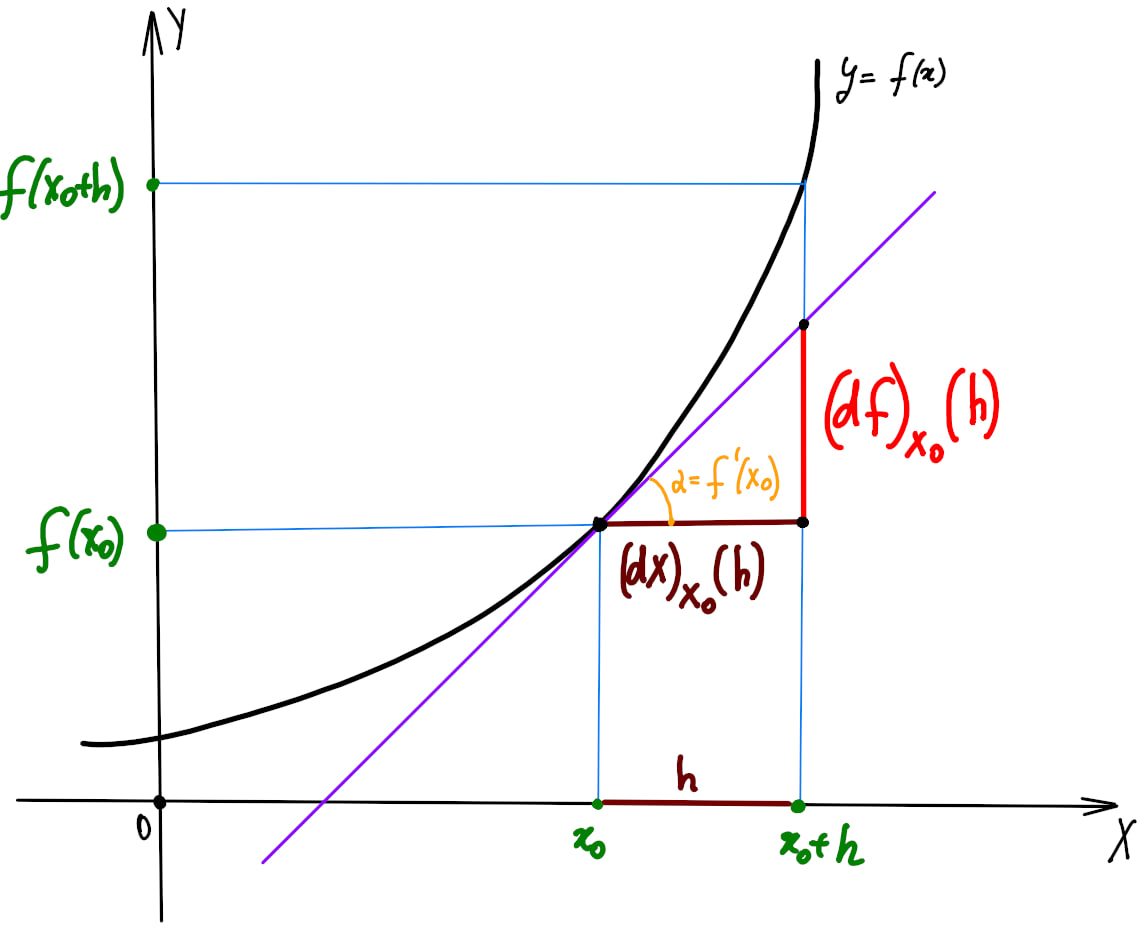
\includegraphics[scale=0.5]{images/df=f'dx.jpg}
    \caption{Caption}
    \label{fig:enter-label}
\end{figure}

При этом, как мы уже знаем, это линейное отображение $(\mathrm{d}f)_{x_0}$ называется дифференциалом функции $f$, вычисленным в точке $x_0$. Более того, имеем равенство
\[
 (\mathrm{d}f)_{x_0}(h): = f'(x_0)\cdot h, 
\]
где мы от $h \in \mathbb{R}$ уже, вообще говоря, ничего не требуем, но если $h\to 0$, то и $(\mathrm{d}f)_{x_0}(h) \to 0.$

Рассмотрим теперь функцию $y(x) = x$, тогда 
\[
 (\mathrm{d}x)_{x_0}(h) = (x'(x_0))\cdot h
\]
и так как $x' = 1$, мы получаем $(\mathrm{d}x)_{x_0}(h) = h$, тогда мы можем записать
\[
 (\mathrm{d}f)_{x_0}(h) = f'(x_0) \cdot h = f'(x_0) \cdot  (\mathrm{d}x)_{x_0}(h).
\]

Тогда мы можем сократить эту формулу следующим образом
\begin{equation}\label{df=f'dx}
  \boxed{
  \mathrm{d}f = f'\cdot \mathrm{d}x.
 }    
\end{equation}


\begin{mydanger}{\bf{!}}
    Нужно понимать, что полученная формула это \textbf{всего лишь соглашение!!!} Ведь эта формула должна пониматься как это написано выше, \textit{т.е.} $(\mathrm{d}f)_{x_0}(h) = f'(x_0) \cdot  (\mathrm{d}x)_{x_0}(h).$    
\end{mydanger}

\begin{remark}
Рассмотрим теперь $\mathbb{R}^n$ cо стандартным базисом $\mathbb{e} = (\m{e}_1,\ldots, \m{e}_n)$, тогда любой вектор $\m{h} = (h_1,\ldots, h_n)^\top  \in \mathbb{R}^n$ записывается в виде $\m{h} = h_1\m{e}_1 + \cdots + h_n \m{e}_n.$ 

Рассмотрим координатные функции 
\[
 x_1,\ldots, x_n:\mathbb{R}^n \to \mathbb{R}, \qquad x_i(\m{h}): = h_i, \quad 1 \le i \le n.
\]

Тогда их дифференциалы $(\mathrm{d}x_1, \ldots, \mathrm{d}x_n)$ -- это в точности базис двойственного пространства $(\mathbb{R}^n)^*$, так как
\[
 (\mathrm{d}x_i)(\m{e}_j) = \delta_{i,j}: = \begin{cases}
     1, & i = j, \\
     0, & i \ne j.
 \end{cases}
\]

Тогда, если $f:\mathbb{R}^n \to \mathbb{R}$ -- дифференцируемая функция в точке $\m{a}$, то её дифференциал (=градиент) можно записать так:
\begin{equation}\label{differential_via_dx}
  \boxed{
 \nabla_\m{a} f = \left.\frac{\partial f}{\partial x_1}\right|_\m{a} \cdot \mathrm{d}x_1 + \cdots +  \left.\frac{\partial f}{\partial x_n}\right|_\m{a} \cdot \mathrm{d}x_n.
    }    
\end{equation}

Действительно, имеем
\begin{eqnarray*}
    (\nabla_\m{a} f) (\m{h}) &=& \left.\frac{\partial f}{\partial x_1}\right|_\m{a} \cdot \mathrm{d}x_1(\m{h}) + \cdots +  \left.\frac{\partial f}{\partial x_n}\right|_\m{a} \cdot \mathrm{d}x_n (\m{h}) \\
    &=& \left.\frac{\partial f}{\partial x_1}\right|_\m{a} \cdot h_1 + \cdots +  \left.\frac{\partial f}{\partial x_n}\right|_\m{a} \cdot h_n ,
   \end{eqnarray*}
   что и есть определение дифференциала фукнции.
\end{remark}

\begin{mydanger}{\bf{!}}
    Это как раз и показывает, что градиент функции есть элемент двойственного пространства, \textit{т.е.} градиент -- это ковектор (=функционал), а не вектор!
\end{mydanger}

\begin{definition}
    Выражение вида 
    \[
     f_1 \mathrm{d}x_1 + \cdots + f_n \mathrm{d}x_n,
    \]
    где $f_1,\ldots, f_n:\mathbb{R}^n \to \mathbb{R}$ -- функции, называется \textit{линейной дифференциальной формой} или \textit{$1$-формой}, и обычно они обозначаются через $\omega$, а пространство всех линейных дифференциальных форм на $\mathbb{R}^n$ обозначается как $\Omega^1(\mathbb{R}^n).$
\end{definition}

\begin{example}
    Дифференциал функции всюду дифференцируемой функции как раз и есть пример дифференциальной формы. Например, пусть $f(x_1,x_2) = x_1^3 - 2x_1x_2 + 3x_2^2$, ясно, что это всюду дифференцируемая функция на $\mathbb{R}^2$. Находим
 \begin{eqnarray*}
   \frac{\partial f}{\partial x_1} &=& 3x_1^2 - 2x_2, \\
   \frac{\partial f}{\partial x_2} &=&  - 2x_1 + 6x_2,
 \end{eqnarray*}

Поэтому, учитывая (\ref{differential_via_dx}), получаем
\[
 \nabla f = (3x_1^2-2x_2)\mathrm{d}x_1 + (-2x_1 + 6x_2) \mathrm{d}x_2.
\]
    
\end{example}




\section{Понятие неопределённого интеграла}

Предыдущий пример доставляет нам множество линейных дифферециальных форм. Возникает естественный вопрос:~

\textit{Пусть нам дана произвольная линейная дифференциальная форма $\omega \in \Omega^1(\mathbb{R}^n)$, существует ли функция $f:\mathbb{R}^n \to \mathbb{R}$ такая, что $\nabla f = \omega$?}

\textbf{Ответом на этот вопрос и занимается теория интегрирования.}

Мы же ограничимся случаем, когда $f$ есть функция от одной переменной, \textit{т.е.} мы будем развивать теорию интегрирования для $\Omega^1(\mathbb{R}).$

Для дальнейшего нам понадобится следующее: 
\begin{definition}
    Промежутком в $\mathbb{R}$ мы называем любое множество, являющееся либо отрезком, либо интервалом, либо полуоткрытым интервалом.
\end{definition}

Понятие неопределённого интеграла возникает при решении следующей задачи:
\textit{пусть мы знаем некоторую функцию $f(x)$, существует ли такая функция $F(x)$, что $F'(x) =f(x)?$}

\begin{definition}\label{int1}
    Функция $F(x)$ в данном промежутке называется \textit{интегралом} (=\textit{первообразной}) для функции $f(x)$, если во всём этом промежутке $f(x)$ является производной для функции $F(x)$ или, что тоже, $f(x)\mathrm{d}x$ есть линейная дифференциальная форма, равная дифференциалу функции $F(x)$
    \[
     F'(x) = f(x) \quad \mbox{или} \quad  \mathrm{d}F = f(x) \mathrm{d}x.
    \]
\end{definition}

\begin{theorem}\label{int1=int2+C}
    Если в некотором промежутке $I \subseteq \mathbb{R}$ функция $F(x)$ есть интеграл для функции $f(x)$, то и функция $F(x) + C$, где $C$ -- любая постоянная (=число), также будет интегралом для $f(x)$. Более того, любые два интеграла $F(x)$, $G(x)$ для одной и той же функции $f(x)$ отличаются на некоторое число $C$, \textit{т.е.} $G(x) =F(x) + C.$
\end{theorem}

\begin{proof}~

(1) Если $F(x)$ -- интеграл для фукнции $f(x)$, то $F'(x) = f(x)$, а тогда
\[
 (F(x) + C)' = F'(x) + (C)' = f(x) + 0 = f(x),
\]
что и означает, что $F(x) +C$ тоже интеграл для $f(x).$

(2) Пусть $F(x), G(x)$ -- два интеграла для фукнции $f(x)$ на промежутке $I$. Пусть $\Phi(x): = F(x) - G(x)$, тогда для любого $x_0 \in I$ имеем $\Phi'(x_0) = 0$. Возьмём (Аксиома Выбора позволяет) другую точку $x \in I$, тогда в зависимости от знака $x_0 - x$ либо $[x_0, x] \subseteq I$, либо $[x,x_0] \in I$. В любом случае, мы имеем выполнение требований теоремы Лагранжа (см. Теорему \ref{Langrange}) для функции $\Phi(x)$. Таким образом, найдётся точка $c \in (x_0, x)$ (\textit{соотв.}, $c \in (x, x_0)$) такая, что
\[
 \Phi(x) - \Phi(x_0) = \Phi'(c)(x-x_0), 
\]
ясно, что $c \in I$, но тогда $\Phi'(c) = 0$, и мы получаем $\Phi(x) = \Phi(x_0) = C$ для любых двух $x,x_0 \in I$. Это завершает доказательство.    
\end{proof}

В силу этого мы вводим следующее определение, которое является очень важным для дальнейшего.

\begin{definition}\label{int2}
    Выражение $F(x) + C$, где $C$ -- произвольная постоянная, представляет собой \textbf{общий вид} функции, которая имеет производную $f(x)$, или её дифференциал есть $1$-форма $f(x) \mathrm{d}x.$

    Это выражение называется \textit{неопределённым интегралом} функции $f(x)$ и обозначается символом
    \[
     \int f(x) \mathrm{d}x,
    \]
    $f(x)$ называется \textit{подынтегральной функцией.}
\end{definition}

\begin{example}
    Пусть $f(x) = x^2$, тогда, как нетрудно догадаться,
    \[
     \int x^2 \mathrm{d}x = \frac{x^3}{3} + C.
     \]
Это легко проверить -- просто дифференцируя правое выражение, мы получим $x^2.$
\end{example}

    
\begin{mydanger}{\bf{!}}
    Ещё раз подчеркнём, что под знаком интеграла $\int$ пишут \textbf{дифференциальную $1$-форму}, а не производную! В предыдущем примере мы писали $\int x^2 \mathrm{d}x$, а не $\int x^2$! Такой способ записи, как будет позже показано, создался исторически; к тому же он представляет целый ряд преимуществ, и его сохранение вполне целесообразно. 
\end{mydanger}

\textbf{Таким образом, интегрируют не функцию $f(x)$, а  дифференциальную 
форму $f(x)\mathrm{d}x$!}

Покажем, что операции $\mathrm{d}$, $\int$ обратны друг к другу.

\begin{lemma}
    \[
     \mathrm{d} \int f(x)\mathrm{d}x = f(x) \mathrm{d}x, \qquad \left( \int f(x) \mathrm{d}x \right)' = f(x).
    \]
\end{lemma}

\begin{proof}
    Пусть $\int f(x) \mathrm{d}x = F(x)+C$, тогда, согласно определению \ref{int1}, $F'(x) = f(x)$, и тогда
    \[
    \left(\int f(x) \mathrm{d}x \right)' =  (F(x) + C)' = F'(x)  = f(x), 
    \]
откуда, согласно (\ref{differential_via_dx}),
\[
 \mathrm{d} \int f(x)\mathrm{d}x = f(x) \mathrm{d}x.
\]
\end{proof}

\begin{lemma}\label{intdF=F}
    Пусть $F(x)$ есть интеграл функции $f(x)$, тогда
    \[
     \int F'(x) \mathrm{d}x = F(x) +C, \qquad \int \mathrm{d}F(x) = F(x) + C.
    \]
\end{lemma}
\begin{proof}
    Если $F(x)$ -- интеграл функции $f(x)$, то согласно определению \ref{int1}, $F'(x) = f(x)$, и тогда
    \[
      \int F'(x) \mathrm{d}x = \int f(x) \mathrm{d}x
    \]
    и по Теореме \ref{int1=int2+C}, получаем
    \[
      \int F'(x) \mathrm{d}x = \int f(x) \mathrm{d}x =  F(x) +C.
    \]
Наконец, так как согласно (\ref{differential_via_dx}), $\mathrm{d}F(x)  = F'(x) \mathrm{d}x$, то используя предыдущие выкладки, мы завершаем доказательство.
\end{proof}

\begin{mydanger}{\bf{!}}
    Не следует пренебрегать такими ``простыми'' наблюдениями! Возможность решать некоторые дифференциальные уравнения появляется благодаря этим двум простым замечаниям! 
\end{mydanger}

\begin{example}
    Так как $(\sin (x))' = \cos(x)$, то мы можем написать
    \[
     \int \cos(x) \mathrm{d}x = \sin(x) +C,
    \]
а так как $(\cos (x))' = -\sin(x)$, то 
\[
 \mathrm{d} \cos(x) =  (\cos (x))'\mathrm{d}x = - \sin(x) \mathrm{d}x.
\]
\textit{т.е.,} мы получаем
\[
 \sin(x) \mathrm{d}x = - \mathrm{d} \cos(x),
 \]
а учитывая, что дифференциал линеен, то мы тогда можем записать последнее равенство так:
\[
 \sin(x) \mathrm{d}x = - \mathrm{d} \cos(x) = \mathrm{d}(-\cos(x)).
 \]
 
Тогда, согласно Лемме \ref{intdF=F},
\[
 \int \sin(x) \mathrm{d}x = \int  \mathrm{d}(-\cos(x)) = -\cos(x) + C.
\]
\end{example}

\begin{proposition}\label{linearity_of_int}
      \[
     \int \Bigl(\alpha f(x) + \beta g(x) \Bigr) \mathrm{d}x = \alpha \int f(x) \mathrm{d}x +\beta \int g(x) \mathrm{d}x,
    \]
    где $\alpha, \beta \in \mathbb{R}.$
\end{proposition}
\begin{proof}
  Пусть $F(x)$, $G(x)$ -- интегралы для фукнции $f(x)$ и $g(x)$, соответственно.
  
(1) Прежде всего, докажем, что 
  \[
   \int \alpha f(x) \mathrm{d}x = \alpha \int f(x) \mathrm{d}x.
  \]

 Если $\alpha = 0$, то мы получаем тождество, поэтому пусть $\alpha \ne 0.$ В силу линейности дифференциала, теоремы \ref{int1=int2+C} и леммы \ref{int2}, получаем
 \begin{eqnarray*}
     \int \alpha f(x) \mathrm{d}x &=& \int \alpha \mathrm{d}F(x) \\
     &=& \int \mathrm{d}(\alpha F(x)) \\
     &=& \alpha F(x) + C \\
     &=& \alpha \left( F(x) + \frac{C}{\alpha} \right).
 \end{eqnarray*}

 Так как $C$ -- произвольное число, то число $\frac{C}{\alpha}$ можно также рассматривать как произвольное, и тогда согласно определению \ref{int2}, выражение в последней скобке -- это $\int f(x) \mathrm{d}x$.

 Получаем
\begin{eqnarray*}
     \int \alpha f(x) \mathrm{d}x &=&\alpha \left( F(x) + \frac{C}{\alpha} \right) \\
     & =& \alpha \int f(x) \mathrm{d}x.
\end{eqnarray*}

(2) Пусть $\alpha, \beta\ne 0$, так как в противном случае, мы либо получаем тождество $0 \equiv 0$, либо что уже было доказано выше.

Используя те же свойства и только что полученное, получаем
\begin{eqnarray*}
    \int \Bigl(\alpha f(x) + \beta g(x) \Bigr) \mathrm{d}x &=& \int\Bigl( \alpha f(x) \mathrm{d}x + \beta g(x) \mathrm{d}x \Bigr) \\
    &=& \int \Bigl( \alpha \mathrm{d}F(x) + \beta \mathrm{d}G(x) \Bigr) \\
    &=& \int \Bigl( \mathrm{d}(\alpha F(x)) + \mathrm{d}(\beta G(x))  \Bigr) \\
    &=& \int \mathrm{d}(\alpha F(x) + \beta G(x)) \\
    &=& \alpha F(x) + \beta G(x) + C.
\end{eqnarray*}

Имеем $C = \frac{C}{2} + \frac{C}{2}$ и так как $C$ -- произвольное число, то и числа $\frac{C}{2\alpha}$, $\frac{C}{2\beta}$ тоже можно считать произвольными. Тогда согласно определению \ref{int2}, линейности дифференциала и леммы \ref{int2}, получаем
\begin{eqnarray*}
    \int \Bigl(\alpha f(x) + \beta g(x) \Bigr) \mathrm{d}x &=& \alpha F(x) + \beta G(x) + C \\
    &=& \alpha \left( F(x) + \frac{C}{2\alpha} \right) + \left(G(x) + \frac{C}{2\beta} \right) \\
    &=&\alpha \int \mathrm{d}F(x) + \beta \int \mathrm{d}G(x) \\
    &=& \alpha \int f(x) \mathrm{d}x + \beta \int g(x) \mathrm{d}x.
\end{eqnarray*}
\end{proof}

\section{Способы интегрирования}

Здесь мы рассмотрим некоторые способы для интегрирования дифференциальных форм от одной переменной. Мы также приведём примеры форм, интегралы от которых невозможно выразить через элементарные функции.

Отметим также, что мы будем говорить об интегралах \textbf{лишь для непрерывных функций}. Если функция задана конкретно и имеет точки разрыва, то рассматривать её будем лишь в промежутках её непрерывности. Поэтому мы освобождаемся от необходимости всякий раз оговаривать существование интегралов: 

\begin{mydanger}{\bf{!}}
    Рассматриваемые нами интегралы все существуют!
\end{mydanger}

\subsection{Замена переменных}

Рассмотрим дифференциальную форму $\omega  = f(x) \mathrm{d}x \in \Omega^1(\mathbb{R})$, и пусть $x$ есть некоторая функция от нового переменного $t$, \textit{т.е.} $x = \varphi(t)$.

\begin{theorem}\label{replace_in_int}
    Если $x = \varphi(t)$ -- дифференцируемая функция на некотором промежутке $I \subseteq \mathbb{R}$, то
    \[
     \int f(x) \mathrm{d}x = \int f(\varphi(t)) \varphi'(t) \mathrm{d}t.
    \]
\end{theorem}
\begin{proof}
 Если $\varphi:\mathbb{R} \to \mathbb{R}$ -- дифференцируемая функция, то мы получаем
\[
 \mathrm{d} x = \mathrm{d} \varphi(t) = \varphi'(t)\mathrm{d}t,
\]
и тогда получаем
\[
 \int f(x) \mathrm{d}x = \int f(\varphi(t)) \varphi'(t) \mathrm{d}t,
\]
что и требовалось доказать.
\end{proof}

\begin{example}
    Покажем, что 
    \[
     \int x^\alpha \mathrm{d}x = \frac{x^{\alpha+1}}{\alpha+1} + C, \qquad \alpha \in \mathbb{R}, \alpha \ne -1.
    \]

Пусть $y(x) = x^{\alpha+1}$, тогда, рассматривая эту функцию в промежутке, в котором она дифференцируема, согласно лемме \ref{intdF=F} имеем
\[
 \int \mathrm{d}y = y+ C' \Longleftrightarrow \int \mathrm{d} x^{\alpha +1} = x^{\alpha +1} + C'.
\]

Далее, $y'(x) = (\alpha +1) x^\alpha$, тогда согласно теореме \ref{replace_in_int}, получаем
\[
 \int \mathrm{d}y = \int (\alpha +1) x^{\alpha} \mathrm{d}x =  x^{\alpha +1} + C'.
\]

Наконец, согласно предложению \ref{linearity_of_int}, получаем
\[
 \int (\alpha +1) x^{\alpha} \mathrm{d}x =  x^{\alpha +1} + C' \Longleftrightarrow (\alpha +1) \int x^\alpha \mathrm{d}x = x^{\alpha +1} + C',
\]
и полагая $C: = \frac{C'}{\alpha +1}$, мы получаем требуемое.
\end{example}


\subsection{Интегрирование по частям}

Докажем следующую формулу, которая называется \textit{правилом интегрирования по частям}.

\begin{theorem}[Интегрирование по частям]
    Пусть $u = u(x)$, $v= v(x)$ -- две функции от $x$, имеющие непрерывные производные $u'= u'(x)$, $v' = v'(x)$. Тогда имеет место формула
    \[
     \int u \mathrm{d}v = uv - \int v \mathrm{d}u.
    \]
\end{theorem}
\begin{proof}

Согласно (\ref{df=f'dx}), а также правилу Лейбница (Теорема \ref{ariph_for_der} 2), имеем 
    \begin{eqnarray*}
        \mathrm{d}(uv) &=& (uv)' \mathrm{d}x \\
        &=& u'v \mathrm{d}x + uv'\mathrm{d}x \\
        &=& v \bigl( u'\mathrm{d}x\bigr) + u \bigl( v'\mathrm{d}x \bigr) \\
        &=& v \mathrm{d}u + u \mathrm{d}v.
    \end{eqnarray*}
Таким образом, $u\mathrm{d}v = \mathrm{d}(uv) - v \mathrm{d}u$. Тогда, используя линейность интеграла (Предложение \ref{linearity_of_int}) и Лемму \ref{intdF=F}, получаем
\begin{eqnarray*}
    \int u \mathrm{d}v &=& \int \Bigl(  \mathrm{d}(uv) - v \mathrm{d}u \Bigr) \\
     &=& \int \mathrm{d}(uv) - \int v \mathrm{d}u \\
     &=& uv - \int v \mathrm{d}u,
\end{eqnarray*}
что и требовалось доказать.    
\end{proof}

\begin{mydanger}{\bf !}
    Следует заметить, что более формально мы должны были бы записать
    \[
    \int \mathrm{d}(uv) - \int v \mathrm{d}u = uv + C - \int v \mathrm{d}u,
    \]
    но выражение $C - \int v \mathrm{d}u$ есть неопределённый интеграл для формы $v\mathrm{d}u$, поэтому его можно записать просто как $\int v \mathrm{d}u.$
\end{mydanger}


\begin{example}
    Рассмотрим типичные примеры на использование этого правила.

    \begin{enumerate}
        \item Рассмотрим форму $\log(x) \mathrm{d}x$, положим $u = \log(x)$ и $v = x$, тогда получаем
\[ 
 \int \log(x) \mathrm{d}x =  \log(x)\cdot x - \int x \mathrm{d}(\log (x)),
 \]
так как $\mathrm{d}(\log(x)) = (\log(x))'\mathrm{d}x = \frac{1}{x}\mathrm{d}x$, то получаем
\begin{eqnarray*}
 \int \log(x) \mathrm{d}x &=& \log(x) \cdot x - \int \frac{x}{x}\mathrm{d}x \\
 &=& x \log(x) - \int \mathrm{d}x \\
 &=& x\log(x) - x + C.   
\end{eqnarray*}
\item Рассмотрим форму $\arctan(x) \mathrm{d}x$, полагая $u = \arctan(x)$, $v = x$, получаем
\[
 \int \arctan(x) \mathrm{d}x = \arctan(x) \cdot x  - \int x \mathrm{d}(\arctan(x)),
\]
так как 
\[
 \mathrm{d}(\arctan(x)) = (\arctan(x))'\mathrm{d}x = \frac{\mathrm{d}x}{1+ x^2},
\]
то получаем
\begin{eqnarray*}
    \int \arctan(x) \mathrm{d}x &=& x \arctan(x) - \int \frac{x\mathrm{d}x}{1+x^2} \\
    &=& x \arctan(x) - \frac{1}{2} \int \frac{\mathrm{d}(x^2)}{1+x^2} \\
    &=& x \arctan(x) - \frac{1}{2} \int \frac{\mathrm{d}(x^2+1)}{1+x^2}\\
    &=& x \arctan(x) - \frac{1}{2} \log(1+x^2) + C.
\end{eqnarray*}
 \item Рассмотрим форму $\omega = x^2 \sin(x) \mathrm{d}x$. Если мы теперь просто положим, что $u = x^2 \sin(x)$, а $v = x$, то, во-первых, мы находим
 \[
  \mathrm{d}u = u'\mathrm{d}x = (x^2 \sin(x))'\mathrm{d}x = 2x \sin(x) \mathrm{d}x + x^2 \cos(x) \mathrm{d}x,
 \]
и тогда мы получаем
\begin{eqnarray*}
  \int x^2 \sin(x) \mathrm{d}x &=& x^3 \sin(x) - \int x \bigl( 2x \sin(x) +x^2 \cos(x)  \bigr)\mathrm{d}x    \\
  &=& x^3 \sin(x) - 2 \int x^2 \sin(x) \mathrm{d}x - \int x^3 \cos(x)  \mathrm{d}x
\end{eqnarray*}
откуда
\[
 \int x^2 \sin(x) \mathrm{d}x = \frac{x^3}{3}\sin(x) -  \int x^3 \cos(x)  \mathrm{d}x.
\]

Таким образом, задача свелась к нахождению интеграла от формы $x^3 \cos(x)\mathrm{d}x$ и если опять положить, что $u= x^3 \cos(x)$, $v = x$, то, как нетрудно проверить, задача уже сведётся к интегрированию формы $x^4 \sin(x)\mathrm{d}x.$

Таким образом, интегрировать первоначальную форму $x^2 \sin(x) \mathrm{d}x$ нужно другим способом. Для этого достаточно вспомнить, что $\mathrm{d}(-\cos(x)) = \sin(x) \mathrm{d}x$. Таким образом, форму можно преобразовать следующим образом
\[
 \omega = x^2 \sin(x) \mathrm{d}x = x \mathrm{d}(-\cos (x)),
\]
тогда, если положить, что $u = x$, а $v = - \cos(x)$, то получаем
 \begin{eqnarray*}
     \int \omega &=& \int u \mathrm{d}(v) = uv - \int v \mathrm{d}u \\
     &=& x (- \cos(x)) - \int (-\cos(x))\mathrm{d}x \\
     &=& - x \cos(x) + \int \cos(x) \mathrm{d}x \\
     &=& - x \cos(x) + \sin(x) +C.
 \end{eqnarray*}
    \end{enumerate}
\end{example}


\section{Интегрирование рациональных функций}

До сих пор мы использовали либо какие-то простые наблюдения, либо какие-то трюки, чтобы интегрировать форму. Разумеется, наукой это назвать нельзя. Здесь мы систематически разработаем технику интегрирования для очень важного класса форм.

\subsection{Элементарные свойства полиномов}

Напомним, что полиномом $P(x)$ от переменной $x$ над $\mathbb{R}$ называется выражение вида 
$$
\alpha_nx^n + \alpha_{n-1}x^{n-1} + \cdots + \alpha_1x + \alpha_0,
$$
где все $\alpha_i \in \mathbb{R}$ и можно положить, что $\alpha_n \ne 0$ и в таком случае говорят, что полином $P(x)$ имеет степень $n$ и пишут $\mathrm{deg}(P(x))= n.$

Множество всех полиномов от переменной $x$ над $\mathbb{R}$ обозначают так: $\mathbb{R}[x].$

\begin{theorem}[Делимость полиномов]\label{div_of_polynmials}
 Для любых полиномов $A(x), B(x) \in \mathbb{R}[x]$ всегда существуют однозначно определённые полиномы $Q(x), R(x) \in \mathbb{R}[x]$ такие, что
 \[
  A(x) = B(x) Q(x) + R(x),
 \]
 и $\mathrm{deg}(R(x)) < \mathrm{deg}(B(x)).$
\end{theorem}
\begin{proof}
    Пусть
    \begin{eqnarray*}
        A(x) &=& \alpha_nx^n + \alpha_{n-1}x^{n-1} + \cdots + \alpha_1x + \alpha_0, \\
        B(x) &=& \beta_kx^k + \beta_{k-1}x^{k-1} + \cdots + \beta_1x + \beta_0,
    \end{eqnarray*}
где $n = \mathrm{deg}(A(x))$, $k = \mathrm{deg}(B(x))$, так что $\alpha_n, \beta_k \ne 0$.

Применим индукцию по $n$.

(1) Если $n =0$ (\textit{т.е.} $A(x) = \alpha_0$) и $0=\mathrm{deg}(A(x)) < \mathrm{deg}(B(x))$, то положим $Q(x):=0$ и $R(x) : = A(x)$, \textit{т.е.} имеем
\[
 \alpha_0 = 0 \cdot B(x) + \alpha_0.
\]

(2) Если $\mathrm{deg}(A(x)) = \mathrm{deg}(B(x)) = 0$, \textit{т.е.} $A(x) = \alpha_0, B(x) = \beta_0$, то положим $R(x) :=0$ и $R(x): = \frac{\alpha_0}{\beta_0}$, \textit{т.е.}
\[
 \alpha_0 = \frac{\alpha_0}{\beta_0} \beta_0 +0.
\]

(3) Пусть теперь $n>0$. Если $\mathrm{deg}(A(x)) < \mathrm{deg}(B(x))$, то положим $Q(x) : = 0$, а $R(x):=A(x).$

Итак, пусть теперь теорема доказана в случае $n>0$ и $\mathrm{deg}(A(x)) \ge \mathrm{deg}(B(x))$. Тогда можем записать
\begin{eqnarray*}
    A(x) &=& \alpha_nx^n + \alpha_{n-1}x^{n-1} + \cdots + \alpha_1x + \alpha_0 \\
    &=& \frac{\alpha_n}{\beta_k} x^{n-k} (\beta_k x^k) + \alpha_{n-1}x^{n-1} + \cdots + \alpha_1x + \alpha_0 \\
    &=& \frac{\alpha_n}{\beta_k} x^{n-k} \Bigl( B(x) - \beta_{k-1}x^{k-1} - \cdots - \beta_0  \Bigr) + \alpha_{n-1}x^{n-1} + \cdots + \alpha_1x + \alpha_0 \\
    &=&  \frac{\alpha_n}{\beta_k}x^{n-k} B(x) + \widetilde{A}(x),
\end{eqnarray*}
где $\mathrm{deg}(\widetilde{A}(x)) = n-1.$ Но тогда по предположению индукции мы можем найти такие $\widetilde{Q}(x)$ и ${R}(x)$, что
\[
 \widetilde{A}(x) = \widetilde{Q}(x)B(x) + {R}(x),
\]
и $\mathrm{deg}((x))< \mathrm{deg}(B(x))$. Тогда получаем
\begin{eqnarray*}
    A(x) &=& \frac{\alpha_n}{\beta_k}x^{n-k} B(x) + \widetilde{A}(x) \\
    &=& \frac{\alpha_n}{\beta_k}x^{n-k} B(x) + \widetilde{Q}(x)B(x) + {R}(x)\\
    &=& Q(x) B(x) + R(x),
\end{eqnarray*}
где $Q(x): = \frac{\alpha_n}{\beta_k}x^{n-k} + \widetilde{Q}(x)$, чем доказательство существования $Q(x)$ и $R(x)$ закончено.

(4) Докажем теперь единственность. Предположим, что
\[
 A(x)  = Q_1(x) B(x) + R_1(x) =  Q_2(x) B(x) + R_2(x),
\]
где $\mathrm{deg}(R_1(x)), \mathrm{deg}(R_2(x)) < \mathrm{deg}(B(x))$. Тогда получаем
\[
\Bigl(Q_1(x) - Q_2(x)\Bigr) B(x) = R_2(x) - R_1(x),
\]
следовательно,
\[
 \mathrm{deg}\left((Q_1(x) - Q_2(x)\Bigr) B(x) \right) = \mathrm{deg}(R_2(x) -R_1(x)),
\]
но
\[
 \mathrm{deg}\left((Q_1(x) - Q_2(x)\Bigr) B(x) \right) = \mathrm{deg}(Q_1(x) - Q_2(x)) + \mathrm{deg}(B(x)),
\]
и так как $\mathrm{deg}(R_2(x) - R_1(x)) < \mathrm{deg}(B(x))$, то последнее равенство возможно лишь в случае, когда $Q_1(x) = Q_2(x)$, \textit{т.е.} $Q_1(x) = Q_2(x)$, и следовательно, $R_1(x) = R_2(x)$, что и требовалось доказать.
\end{proof}

Мы считаем известными (или мы просто их принимаем) следующие два факта из алгебры:

\begin{theorem}[{Основная теорема алгебры}]
    Всякое уравнение
    \[
     \alpha_n x^n + \alpha_{n-1}x^{n-1} + \cdots + \alpha_1 x + \alpha_0 =0,
    \]
    где все $\alpha_i \in \mathbb{C}$, $n\ge 1$, $\alpha_n \ne 0$ имеет по крайней мере один комплексный корень.
\end{theorem}

\begin{theorem}[{Теорема Безу}]
    Если $a$ -- корень уравнения 
        \[
     \alpha_n x^n + \alpha_{n-1}x^{n-1} + \cdots + \alpha_1 x + \alpha_0 =0,
    \]
    то полином $P(x) = \alpha_n x^n + \alpha_{n-1}x^{n-1} + \cdots + \alpha_1 x + \alpha_0 =0$ делится без остатка на полином $x-a.$
\end{theorem}


Тогда мы получаем очень важное для нас следствие:

\begin{theorem}\label{any_polynomail_is_1+2}
    Любой полином $P(x)$, $\mathrm{deg}(P(x)) \ge 1$ с действительными коэффициентами может быть представлен в виде
    \[
     P(x) = (x - a_1)^{k_1} \cdots (x-a_p)^{k_p} (x^2 + b_1x + c_2)^{m_1}\cdots (x^2 + b_qx + c_q)^{m_q}, 
    \]
    где $k_1 + \cdots + k_p + 2m_1 + \cdots + 2m_q = \mathrm{deg}(P(x))$ и все $k_i, m_j \in \mathbb{Z}_{\ge 0}.$
\end{theorem}

\begin{proof}
Согласно теореме Безу, нужно просто доказать, что любой полином $P(x) \in \mathbb{R}[x]$ делится либо на линейный полином вида $(x-a)$, либо на квадратный $(x^2 + bx + c)$. Но по теореме Безу, если $P(x)$ имеет корень $a$, то $P(x)$ делится на $(x-a)$, потому все числа $a_1,\ldots, a_p$ -- это просто все корни уравнения $P(x) = 0$.
    
Далее, рассмотрим теперь $P(x)$ как полином в множестве $\mathbb{C}[x]$, это возможно, потому что $\mathbb{R} \subset \mathbb{C}$. Тогда по основной теореме алгебры существует комплексное число $\zeta = \alpha + \beta \sqrt{-1}$, что $P(z) =0$. Тогда по теореме Безу $P(x)$ делится на $(x- \alpha - \beta \sqrt{-1})$.
    
Пусть $P(x) = \alpha_nx^n + \cdots + \alpha_1 x + \alpha_0$, тогда если $P(\zeta) =0$, где $\zeta \in \mathbb{C}$, то получаем
\begin{eqnarray*}
    P(\overline{\zeta}) &=&  \alpha_n {\overline{\zeta}}^n + \cdots + \alpha_1 \overline{\zeta} + \alpha_0 \\
    &=& \overline{\alpha_n \zeta^n} + \cdots + \overline{\alpha_1 \zeta} + \overline{\alpha_0} \\
    &=& \overline{\alpha_nx^n + \cdots + \alpha_1 x + \alpha_0} \\
    &=& \overline{P(\zeta)} = 0.
\end{eqnarray*}

Это означает, что $\overline{\zeta}$ тоже является корнем уравнения $P(x) = 0$, тогда по теореме Безу $P(x)$ делится на $x - \overline{\zeta} = x - (\alpha -\beta \sqrt{-1})$.

Таким образом, полином $P(x)$ делится на произведение $(x - \zeta)(x - \overline{\zeta})$.

Находим
\[
 (x - \zeta)(x - \overline{\zeta}) = (x - \alpha - \beta \sqrt{-1})(x - \alpha + \beta \sqrt{-1}) = x^2 - 2 \alpha x + \alpha^2 + \beta^2,
\]
\textit{т.е.} полином $P(x)$ делится на полином второй степени. Это завершает доказательство. 
\end{proof}


\subsection{Рациональная функция и её разложение}

Мы умеем интегрировать формы вида $P(x) \mathrm{d}x$, где $P(x)$ -- полином, сейчас мы хотим развить теорию интегрирования форм вида $\frac{P(x)}{Q(x)}\mathrm{d}x$, где $Q(x)$ тоже полином и всегда подразумевается, что $Q(x) \ne 0$. 

Выражения вида $\frac{P(x)}{Q(x)}$ называются \textit{дробями}, и как и в случае числовых дробей, целесообразно рассматривать так называемые несократимые дроби. Формализацией этого желания является следующее определение. 

\begin{definition}
    Рациональная функция от одной переменной -- это класс эквивалентности дробей вида $\dfrac{P(x)}{Q(x)}$, где $P(x), Q(x)$ -- полиномы, $Q(x) \ne 0$, и мы считаем, что две такие дроби эквивалентны
    \[
     \frac{P(x)}{Q(x)} \sim \frac{A(x)}{B(x)},
    \]
    если и только если $P(x) B(x) = A(x) Q(x).$
\end{definition}

Множество всех рациональных функций образует поле \footnote{Доказательство этого факта очевидно и при этом банальное, нужно лишь проверить выполнение аксиом i.1 -- i.9 определения поля (см. Определение \ref{field}).}, которое так и называется \textit{полем рациональных функций} и обозначается так: $\mathbb{R}(x).$

\begin{remark}\textit{
  Более того, можно пойти дальше и рассматривать поля рациональных функций от нескольких переменных, \textit{т.е.} выражений вида $\frac{P(x,y)}{Q(x,y)}$, где $P(x,y)$, $Q(x,y)$ -- полиномы от двух переменных. Оказывается, что если мы ограничим множество рассматриваемых полиномов, например, чтобы знаменатель не делился на какой-то конкретный полином $F(x,y)$, то мы получаем поле рациональных функций на кривой, заданной уравнением $F(x,y)=0$. Это поле является очень важной характеристикой кривой. Более того, как мы увидим далее, именно изоморфизм полей у кривых позволяет сводить сложные интегралы к более простым. Поэтому неудивительно, что в теории интегрирования столько алгебры. }   
\end{remark}

Так как имеется процесс деления полиномов друг на друга, то введём следующее понятие:

\begin{definition}
    Дробь $\frac{P(x)}{Q(x)}$ называется \textit{правильной}, если $\mathrm{deg}(P(x)) < \mathrm{deg}(Q(x))$.
\end{definition}

\begin{mydanger}{\bf !}
    Если дробь неправильная, то, поделив числитель на знаменатель (теорема \ref{div_of_polynmials}), мы получим полином плюс правильная дробь. Это аналогично выделению целой части в неправильной числовой дроби.
\end{mydanger}


Используя теперь теорему \ref{any_polynomail_is_1+2}, мы можем разложить знаменатель на более простые множители. Оказывается, это влечёт разложение и самой дроби. Введём следующее понятие.

\begin{definition}
    \textit{Простыми} дробями в поле $\mathbb{R}(x)$ называются выражения вида
    \begin{enumerate}
        \item $\dfrac{A}{(x-\alpha)^k}$, где $A,\alpha \in \mathbb{R}$, и $k\ge 1$,
        \item $\dfrac{Ax + B}{(x^2 + ax + b)^n}$, где $A,B, a,b \in \mathbb{R}$, $n\ge 1$ и предполагается, что $x^2 + ax +b$ не имеет вещественных корней.
    \end{enumerate}
    \end{definition}


\begin{theorem}\label{decomp_of_fraction}
    Каждая правильная дробь может быть представлена в виде суммы конечного числа простых дробей.
\end{theorem}
\begin{proof}
Рассмотрим дробь $\frac{P(x)}{Q(x)}$, согласно теореме \ref{any_polynomail_is_1+2}, мы можем записать знаменатель в виде 
 \[
 Q(x) = (x - a_1)^{k_1} \cdots (x-a_p)^{k_p} (x^2 + b_1x + c_2)^{m_1}\cdots (x^2 + b_qx + c_q)^{m_q}, 
    \]
    где $k_1 + \cdots + k_p + 2m_1 + \cdots + 2m_q = \mathrm{deg}(P(x))$ и все $k_i, m_j \in \mathbb{Z}_{\ge 0}$, и более того, согласно теореме Безу, все $a_i$ -- это всё корни уравнения $Q(x) =0.$

(1) Пусть хотя бы один $k_i$ больше нуля, обозначим его просто через $k$, тогда можно записать $Q(x) = (x-a)^k \widetilde{Q}(x)$, где $a$ -- это соответствующее число из чисел $a_i$. Тогда $a$ не является корнем уравнения $\widetilde{Q}(x) =0.$

Допустим теперь, что существует такое число $A$ и такой полином $\widetilde{P}(x)$, что 
\[
 \frac{P(x)}{Q(x)} = \frac{A}{(x-a)^k} + \frac{\widetilde{P}(x)}{(x-a)^{k-1}\widetilde{Q}(x)}.
\]

Для доказательства этого равенства достаточно подобрать эти неизвестные $A, \widetilde{P}(x)$ так, чтобы выполнялось равенство
\[
 P(x) - A \widetilde{Q}(x) = (x-a)\widetilde{P}(x).
\]

Так как $A$ это число, то оно не должно зависеть от $x$, поэтому положим в этом равенстве $x = a$, и тогда мы получаем, что
\[
 P(a) - A \widetilde{Q}(a) = 0
\]
откуда $A = \frac{P(a)}{\widetilde{Q}(a)}$. Это выражение корректно, так как $a$ был выбран так, чтобы $a$ -- корень уравнения $Q(x) =0$, но не корень уравнения $\widetilde{Q}(x) = 0.$

Далее, полином $\widetilde{P}(x)$ можно теперь определить следующим образом:
\[
 \widetilde{P}(x): = \frac{P(x) - A \widetilde{Q}(x)}{x-a}.
\]

(2) Пусть теперь $Q(x)$ содержит хотя бы один сомножитель вида $(x^2 + bx + c)^m$, тогда запишем $Q(x)= (x^2 + bx + c)^m \widehat{Q}(x)$, где уже $\widehat{Q}(x)$ не делится на $x^2 + bx + c$. Тогда подберём числа $B,C$ и полином $\widehat{P}(x)$ так, чтобы
\[
 \frac{P(x)}{Q(x)} = \frac{Bx + C}{(x^2 + bx + c)^m} + \frac{\widehat{P}(x)}{(x^2 + bx + c)^{m-1} \widehat{Q}(x)}.
\]

Это то же самое, что подобрать эти же неизвестные, чтобы выполнялось равенство
\[
 P(x) - (Bx +C)\widehat{Q}(x) = (x^2 + bx + c) \widehat{P}(x).
\]

Поступим следующим образом. Разделим полиномы $P(x)$, $\widehat{Q}(x)$ на $x^2 + bx + c$ с остатком;
\begin{eqnarray*}
    P(x) &=& F(x)(x^2 + bx + c) + \alpha x + \beta, \\
    \widehat{Q}(x) &=& H(x)(x^2 + bx + c) + \gamma x + \delta.
\end{eqnarray*}

Тогда, подставляя в предыдущее равенство, получаем
\[
 F(x)(x^2 + bx + c) + \alpha x + \beta - (Bx +C) \bigl( H(x)(x^2 + bx + c) + \gamma x + \delta\bigr) = (x^2 + bx + c) \widehat{P}(x).
\]

Потребуем теперь, чтобы полином
\[
 R(x) = \alpha x + \beta  - (Bx + C) (\gamma x +\delta ) =0
\]
делился на $x^2 + bx + c$ без остатка.

\begin{mydanger}{\bf !}
 Если можно будет найти такие числа, то значит, мы добьёмся того, что существуют такие $B,C$, что полином $P(x) - (Bx + C)\widehat{Q}(x)$ делится на $x^2 + bx + c$ без остатка. В таком случае, полином $\widehat{P}(x)$ находится как частное от деления полинома $P(x) - (Bx + C)\widehat{Q}(x)$ на $x^2 + bx + c$.  
\end{mydanger}

Итак, имеем
\begin{eqnarray*}
    R(x) &=& \alpha x + \beta  - (Bx + C) (\gamma x +\delta )  \\
    &=& - \gamma B x^2 + (\alpha - \delta B - \gamma C)x + (\beta - \delta C).
\end{eqnarray*}

Разделив теперь $R(x)$ на $x^2 + bx +c $ на $x^2 + bx +c$, мы получим в остатке следующее выражение:

\[
 \Bigl( (b \gamma - \delta)B - \gamma C  + \alpha \Bigr)x + c \gamma B - \delta C + \beta.
\]

Тогда мы получаем систему (относительно неизвестных $B,C$) линейных уравнений
\[
 \begin{cases}
     (b \gamma - \delta)B - \gamma C =- \alpha \\
      c \gamma B - \delta C =- \beta.
 \end{cases}
\]

Определитель этой системы имеет вид
\[
\Delta = \begin{vmatrix}
     b \gamma - \delta & \gamma \\
     c\gamma & -\delta
 \end{vmatrix} = \delta^2 - b\gamma \delta + c \gamma^2
\]

Пусть $\gamma \ne 0$, тогда
\[
 \Delta = \gamma^2 \left( \left( -\frac{\delta}{\gamma} \right)^2 + b \left(-\frac{\delta}{\gamma}\right) + c \right),
\]
но это есть значение полинома $x^2 + bx +c$ в точке $x = -\frac{\delta}{\gamma}$ и, следовательно $\Delta \ne 0$, ибо мы предположили, что $x^2 + bx +c$ не имеет корней. Таким образом, система имеет решение, и числа с необходимым требованием существуют. 

Если же $\gamma =0$, то $\Delta = \delta^2$, но так как $\widehat{Q}(x) = H(x)(x^2 + bx + c) + \gamma x + \delta$, то $\delta \ne 0$ ибо $\widehat{Q}(x)$ на $x^2 + bx +c$ не делится.

Итак, в любом случае, решение системы существует, а значит, можно подобрать так $B,C$, чтобы полином $P(x) - (Bx + C)\widehat{Q}(x)$ делится на $x^2 + bx + c$ без остатка. В таком случае полином
\[
 \widehat{P}(x): = \frac{P(x) - (Bx + C)\widehat{Q}(x}{x^2 + bx + c}.
\]

Таким образом, доказательство теоремы сводится к повторному применению случаев (1) и (2), которые обеспечивают возможность последовательного выделения простых дробей из данной правильной дроби, вплоть до её исчерпывания. Это доказывает теорему.
\end{proof}





\begin{lemma}\label{int_of_(x-a)^{-k}}
    \[
     \int \frac{A}{(x-\alpha)^k} \mathrm{d}x = \begin{cases}
         A \log|x-\alpha| + C, & k =1,\\
         - \frac{A}{k-1}\cdot \frac{1}{(x-\alpha)^{k-1}} + C, & k >1.
     \end{cases}
    \]
\end{lemma}
\begin{proof}
    С помощью замены $y =x-\alpha$ интегрирование формы $\omega = \frac{A}{(x-\alpha)^k}$ сводится к интегрированию формы $\frac{A}{y^k}$, что и даёт нужный результат, так как $\mathrm{d}y = \mathrm{d}(x-\alpha) = \mathrm{d}x.$
\end{proof}

Чтобы научится интегрировать форму $\dfrac{Ax + B}{(x^2 + ax + b)^n} \mathrm{d}x$, нам нужно сначала научится интегрировать форму $\dfrac{\mathrm{d}x}{(x^2 + \alpha^2)^n}.$

\begin{lemma}\label{int_of_x^2+a^2}
    Для каждого $n\ge 1$ рассмотрим форму
    \[
     \omega_n: = \frac{\mathrm{d}x}{(x^2 + \alpha^2)^n},
    \]
    тогда
    \[
     \int \omega_{n+1} = \frac{1}{2n\alpha^2}\cdot \frac{x}{(x^2 + \alpha^2)^n} + \frac{2n-1}{2n\alpha^2} \cdot\int \omega_n, \qquad \int \omega_1 = \frac{1}{\alpha} \cdot \arctan\left( \frac{x}{\alpha}\right) + C.
    \]
\end{lemma}
\begin{proof}~

(1) Так как $(\arctan(y))' = \frac{1}{y^2 + 1}$, то
\begin{eqnarray*}
    \int \omega_1 &=& \int \frac{\mathrm{d}x}{x^2 + \alpha^2}  = \bigintss \frac{\mathrm{d}x}{\alpha^2\cdot\left (\left( \frac{x^2}{\alpha^2} \right) + 1\right)}\\
    &=& \frac{1}{\alpha^2} \bigints \frac{\alpha \cdot\mathrm{d}\left(\frac{x}{\alpha}\right)}{\left( \frac{x^2}{\alpha^2} \right) + 1} = \frac{1}{\alpha} \bigints \frac{ \mathrm{d}\left(\frac{x}{\alpha}\right)}{\left( \frac{x}{\alpha} \right)^2 + 1} = \frac{1}{\alpha} \cdot \arctan\left( \frac{x}{\alpha}\right) + C.
\end{eqnarray*}

(2) Пусть теперь $n \ge 1$, будем интегрировать $\omega_n$ по частям, \textit{т.е.} воспользуемся правилом
\[
 \int u \mathrm{d}v = uv - \int v \mathrm{d}u.
\]

Положили $u = \frac{1}{(x^2 + \alpha^2)^n}$, $v = x$, находим
\[
 \mathrm{d}u = \left( \frac{1}{(x^2 + \alpha^2)^n} \right)'\mathrm{d}x = - \frac{2nx}{(x^2 + \alpha^2)^{n+1}}\mathrm{d}x, \qquad \mathrm{d}v = \mathrm{d}x.
\]

Тогда
\begin{eqnarray*}
    \int \omega_n &=& \int \frac{\mathrm{d}x}{(x^2 + \alpha^2)^n} = \frac{x}{(x^2 + \alpha^2)^n} + 2n \cdot \int \frac{x^2}{(x^2 + \alpha^2)^{n+1}}\mathrm{d}x \\
    &=& \frac{x}{(x^2 + \alpha^2)^n} + 2n \cdot \int \frac{(x^2+\alpha^2) - \alpha^2}{(x^2 + \alpha^2)^{n+1}}\mathrm{d}x \\
    &=& \frac{x}{(x^2 + \alpha^2)^n} + 2n \cdot \left( \int \frac{(x^2+\alpha^2)}{(x^2 + \alpha^2)^{n+1}}\mathrm{d}x - \alpha^2 \int  \frac{\mathrm{d}x}{(x^2 + \alpha^2)^{n+1}}\right) \\
    &=& \frac{x}{(x^2 + \alpha^2)^n} + 2n \cdot \left( \int \frac{\mathrm{d}x}{(x^2 + \alpha^2)^{n}} - \alpha^2 \int  \frac{\mathrm{d}x}{(x^2 + \alpha^2)^{n+1}}\right) \\
    &=&\frac{x}{(x^2 + \alpha^2)^n} + 2n\cdot \int \omega_n  - 2n\alpha^2 \int \omega_{n+1},
\end{eqnarray*}
\textit{т.е.} мы получили рекуррентное соотношение 
\[
 \int \omega_n = \frac{x}{(x^2 + \alpha^2)^n} + 2n\cdot \int \omega_n  - 2n\alpha^2 \int \omega_{n+1},
\]
из которого и следует требуемое.    
\end{proof}


\begin{lemma}\label{int_of_prime} Интеграл от формы $\frac{Ax + B}{(x^2 + ax + b)^n}\mathrm{d}x$ выражается через рациональные функции и функции $\log$, $\arctan$.
\end{lemma}
\begin{proof}
Выделим в выражении $x^2 + ax + b$ полный квадрат
\[
 x^2 + ax + b = \left(x+ \frac{a}{2} \right)^2 + \left(b - \frac{a^2}{4} \right),
\]
так как по условию $x^2 + ax + b =0$ не имеет корней, то $a^2 - 4b <0$, тогда положим 
\[
 c^2: = b- \frac{a^2}{4}, \qquad c = + \sqrt{b- \frac{a^2}{4}}
\]
тогда сделаем замену 
\[
y:= x+ \frac{a}{2},
\]
находим
\begin{eqnarray*}
    \mathrm{d}y &=& \left( x+ \frac{a}{2}\right)' \mathrm{d}x = \mathrm{d}x,\\
    x^2 + ax + b &=& \left(x+ \frac{a}{2} \right)^2 + \left(b - \frac{a^2}{4} \right) = y^2 + c^2, \\
    Ax + B &= & Ay + \left(B - \frac{Aa}{2} \right).
\end{eqnarray*}

Рассмотрим два случая.

(1) $n = 1$, тогда получаем
\begin{eqnarray*}
    \int \frac{Ax + B}{x^2 + ax + b}\mathrm{d}x = \bigintss \frac{Ax + \left( B - \frac{Aa}{2} \right)}{y^2 + c^2}\mathrm{d}y &=& \frac{A}{2} \int \frac{2y\mathrm{d}y}{y^2 + c^2} + \left( B - \frac{Aa}{2} \right) \int \frac{\mathrm{d}y}{y^2 + c^2} \\
    &=& \frac{A}{2} \log(y^2 + c^2) + \frac{1}{c} \cdot \left( B - \frac{Aa}{2} \right)\arctan\left(\frac{y}{c}\right) + C,
\end{eqnarray*}
или, возвращаясь к $x$ и подставляя вместо $c$ его значение:
  \[
   \bigintsss \frac{Ax + B}{x^2 + ax + b}\mathrm{d}x =  \frac{A}{2}\log(x^2 + ax + b) + \frac{2B-Aa}{\sqrt{4b-a^2}}\arctan\left( \frac{2x+a}{\sqrt{4b-a^2}} \right) + C.
  \]

(2) Пусть $n >1$, делая ту же замену, получаем
\[
    \int \frac{Ax + B}{(x^2 + ax + b)^n}\mathrm{d}x = \bigintss \frac{Ax + \left( B - \frac{Aa}{2} \right)}{(y^2 + c^2)^n}\mathrm{d}y = \frac{A}{2} \int \frac{2y\mathrm{d}y}{(y^2 + c^2)^n} + \left( B - \frac{Aa}{2} \right) \int \frac{\mathrm{d}y}{(y^2 + c^2)^n}.
\]

Видим, что второй интеграл это интеграл от формы $\omega$ который найден в лемме \ref{int_of_x^2+a^2}, первый же интеграл легко берётся с помощью замены $t:=y^2 + c^2 $, тогда $\mathrm{d}t = (y^2 + c^2)'\mathrm{d}y = 2y\mathrm{d}y$, следовательно $y\mathrm{d}y = \frac{1}{2}\mathrm{d}t$, и мы получаем
\[
 \int \frac{2y\mathrm{d}y}{(y^2 + c^2)^n} = \int \frac{\mathrm{d}t}{t^n} = - \frac{1}{n-1}\cdot \frac{1}{t^{n-1}} +C.
\]
Тем самым лемма доказана.
\end{proof}

\begin{theorem}\label{int_of_rational}
    Интеграл от формы вида $\frac{P(x)}{Q(x)}$ выражается через рациональные функции и функции $\log, \arctan.$ 
\end{theorem}

\begin{proof}
    Действительно, если дробь не правильная, то поделив $P(x) = B(x) Q(x) + R(x)$ на $Q(x)$ мы получаем
    \[
     \int \frac{P(x)}{Q(x)}\mathrm{d}x = \int B(x)\mathrm{d}x + \int \frac{R(x)}{Q(x)}\mathrm{d}x.
    \]

Первый интеграл находится легко, так как это интеграл от полинома, а во втором интеграле присутствует уже правильная дробь. Но согласно теореме \ref{decomp_of_fraction} каждая правильная дробь представляется в виде суммы простых, тогда из лемм \ref{int_of_(x-a)^{-k}}, \ref{int_of_prime} вытекает утверждение теоремы.    
\end{proof}

\subsection{Интегрирование форм, содержащих радикалы}

В этом разделе мы рассмотрим формы вида 
\[
 R\left(x, \left(\frac{ax+b}{a'x+b'} \right)^{r_1}, \ldots, \left(\frac{a'x+b'}{cx+d} \right)^{r_n} \right)\mathrm{d}x,
\]
где $R(x_1,y_1,\ldots, y_n)$ -- рациональная функция от переменных $x_1,y_1,\ldots, y_n,$ $m,n \in \mathbb{Z}$, а $r_i, p \in \mathbb{Q}.$ 

\begin{example}
 Пусть, например $R(x,y) \in \mathbb{R}(x,y)$ -- рациональная функция от двух переменных $x,y$, имеющая вид
\[
 R(x,y) = \frac{y+2}{(x+1)^2 -y},
\]
тогда если мы рассмотрим форму
\[
 \omega = \frac{\sqrt{x+1}  +2}{(x+1)^2 - \sqrt{x+1}}\mathrm{d}x,
\]
то видно, что $\omega = R(x, \sqrt{x+1})\mathrm{d}x.$
\end{example}

\begin{mydanger}{\bf !}
    Но некоторые формы не всегда имеют такой очевидный вид как в предыдущем примере.
\end{mydanger}

\begin{example}
    Рассмотрим форму
    \[
     \omega = \frac{\mathrm{d}x}{\sqrt[3]{(x-1)(x+1)^2}}.
    \]
    В таком виде её уже нельзя представить как $R(x,y)\mathrm{d}x$, однако сделаем следующие преобразования
    \begin{eqnarray*}
     \omega  &=&  \frac{\mathrm{d}x}{\sqrt[3]{(x-1)(x+1)^2}} \\
     &=&  \frac{\mathrm{d}x}{\sqrt[3]{(x-1)\frac{(x+1)^3}{(x+1)} }} \\
     &=&  \frac{\mathrm{d}x}{(x+1) {\sqrt[3]{\frac{x-1}{x+1}}}} \\
     &=& \sqrt[3]{\frac{x+1}{x-1}}\cdot \frac{1}{x+1}\mathrm{d}x, \\
    \end{eqnarray*}
и тогда уже можно написать, что $\omega = R(x,y)\mathrm{d}x$, где $R(x,y) = \frac{y}{x+1}$.
\end{example}

\begin{theorem}
Пусть $R(x,y_1,\ldots, y_n)$ -- рациональная функция. Для любых рациональных чисел $r_1, \ldots, r_n \in \mathbb{Q}$ и любых $a,b,a',b' \in \mathbb{R}$, $a',b'\ne 0$ интеграл
 \[
  \bigintss R\left(x, \left(\frac{ax+b}{a'x+b'} \right)^{r_1}, \ldots, \left(\frac{ax+b}{a'x+b'} \right)^{r_n} \right)\mathrm{d}x
 \]
 выражается через рациональные функции и функции $\log, \arctan.$
\end{theorem}
\begin{proof}
Ясно, что без ограничения общности можно считать, что все $r_i$ положительные. Пусть $r_1 = \frac{p_1}{q_1}, \ldots, r_n = \frac{p_n}{q_n}$, и пусть $q:=q_1,\ldots, q_n$, тогда
\[
 q_i = \frac{q }{q_1 \cdots \widehat{q_i}\cdots q_n},
\]
где $\widehat{q_i}$ означает, что в выражении $q_1\cdots q_n$ число $q_i$ пропущено.

Сделаем тогда замену 
    \[
     u: = \left(\frac{ax + b}{a'x + b'} \right)^{\frac{1}{q}},
    \]
    тогда получаем для каждого $1\le i \le n$
    \[
    \left( \frac{ax+b}{a'x + b'} \right)^{\frac{p_i}{q_i}} =  \left( \frac{ax+b}{a'x + b'} \right)^{\frac{p_i\cdot q_1 \cdots \widehat{q_i}\cdots q_n}{q}} = u^{p_i\cdot q_1 \cdots \widehat{q_i}\cdots q_n} = u^{k_i},
    \]
где $k_i : = p_i\cdot q_1 \cdots \widehat{q_i}\cdots q_n \in \mathbb{N}$. Таким образом, получаем
\[
 R\left(x, \left(\frac{ax+b}{a'x+b'} \right)^{r_1}, \ldots, \left(\frac{ax+b}{a'x+b'} \right)^{r_n} \right) = R(x,u^{k_1},\ldots, u^{k_n}),
\]
\textit{т.е.} мы избавились от иррациональности (=радикалов) в самой функции. Посмотрим тогда, что произойдёт с формой. Для этого нужно выразить $\mathrm{d}x$ через $\mathrm{d}u.$

Так как $u^q = \frac{ax + b}{a'x+b'}$, то $x = \frac{b'u^q - b}{a - a'u^q}$, а тогда 
\[
 \mathrm{d}x = \left(\frac{b'u^q - b}{a - a'u^q} \right)'_u\mathrm{d}u,
\]
но ведь производная этой дроби тоже рациональная функция от $u$. Таким образом, интегрирование изначальной формы свелось к интегрированию формы вида $\widetilde{R}(u)\cdot\left(\frac{b'u^q - b}{a - a'u^q} \right)'\mathrm{d}u$, где 
\[
 \widetilde{R}(u): = R\left( \frac{b'u^q- b}{a- a'u^q}, u^{k_1}, \ldots, u^{k_n} \right)
\]
рациональная функция от одной переменной $u.$ Но тогда, воспользовавшись теоремой \ref{int_of_rational}, мы завершаем доказательство.
\end{proof}


\begin{example}
    Найдём 
    \[
     \bigintsss \frac{\sqrt{x}}{\sqrt[4]{x^3} +4} \mathrm{d}x.
    \]
Мы можем положить, что $x = u^4$, так как $4$ -- наименьшее общее кратное для $2,4$. Тогда находим $\mathrm{d}x = (u^4)'\mathrm{d}x = 4u^3 \mathrm{d}u$, подставляем
\begin{eqnarray*}
    \bigintsss \frac{\sqrt{x}}{\sqrt[4]{x^3} +4} \mathrm{d}x &=& \bigintsss \frac{x^{\frac{1}{2}}}{x^{\frac{3}{4}}+4} \mathrm{d}x \\
    &=& 4 \bigintsss \frac{u^2 \cdot u^3 \mathrm{d}u}{u^3+4} = 4 \bigintsss \frac{u^5\mathrm{d}u}{u^3+4} \\
    &=& 4 \bigintsss \left(u^3 - \frac{4u^2}{u^3+4} \right)\mathrm{d}u \\
    &=& 4\bigintsss u^3 \mathrm{d}u - 16 \bigintsss\frac{u^2 \mathrm{d}u}{u^3 +4} = 4\bigintsss u^3 \mathrm{d}u - \frac{16}{3} \bigintsss\frac{\mathrm{d}(u^3)}{u^3 +4} \\
    &=& u^4 - \frac{16}{3} \log |u^3 + 4| +C,
\end{eqnarray*}
и тогда
 \[
     \bigintsss \frac{\sqrt{x}}{\sqrt[4]{x^3} +4} \mathrm{d}x = \sqrt[4]{x^3} - \frac{16}{3} \log \left| \sqrt[4]{x^3} + 4 \right| + C.
    \]
\end{example}




